% !TEX root = ../MA119-Main.tex

\paragraph*{The Slope-Intercept Form Equation}
	The slope of a line measures the steepness, in other words, ``rise'' over ``run'', or rate of change of the line. Using the rectangular coordinate  system, the \dfn{slope} $m$ of a line is defined as
	$$
	m=\dfrac{y_2-y_1}{x_2-x_1}=\dfrac{\textup{rise}}{\textup{run}}=\dfrac{\text{change in the output }y}{\text{change in the input } x},
	$$
	where $(x_1, y_1)$ and $(x_2, y_2)$ are any two distinct points on the line. If the line intersects the $y$-axis at the point $(0, b)$, then a point $(x, y)$ is on the line if and only if
	$$
	y=mx+b.
	$$
	This equation is called the \dfn{slope-intercept form} of the line.


\paragraph*{Point-Slope Form Equation of a Line}

		Suppose a line passing through the point $(x_0, y_0)$ has the slope $m$. Solving from the slope formula, we see that any point $(x, y)$ on the line satisfies the equation equation
		$$
		y=m(x-x_0)+y_0
		$$
		which is called the \dfn{point-slope form} equation.

\paragraph*{Linear Function}

	A \dfn{linear function} $f$ is a function whose graph is a line. An equation for $f$ can be written as
	$$f(x) = mx + b$$
	where $m$ is the slope and $b=f(0)$.

	A function $f$ is a linear function if the following equalities hold
	$$
	\dfrac{f(x_2)-f(x_1)}{x_2-x_1}
	=\dfrac{f(x_3)-f(x_1)}{x_3-x_1}
	$$
	for any three distinct points $(x_1, y_1)$, $(x_2, y_2)$ and $(x_3, y_3)$ on the graph of $f$.



\paragraph*{How to Write an Equation for a Linear Function?}

\mbox{}

	\begin{example}
		Find the slope-intercept form equation for the linear function $f$ such that $f(2)=5$ and $f(-1) = 2$.
	\end{example}

	\begin{solution}	
	\begin{enumerate}[label={\textbf{\textup{Step \arabic*.}}~}, itemsep=0em]
			\item Find the slope $m$: $m=\frac{f(2)-f(-1)}{2-(-1)}=\frac{5-2}{2-(-1)}=\frac{3}{3}=1$.
			\item Plug one of the points, say $(2, 5)$ in the point-slope form equation, we get $y=1\cdot(x-2)+5$
			\item Simplify the above equation, we get the slope-intercept form equation $f(x)=x+3$.
		\end{enumerate}
	\end{solution}



\paragraph*{Graph a Linear Function by Plotting Points}

\mbox{}


	\begin{example}
		Sketch the graph of the linear function $f(x)=-\frac12 x + 1$.	
	\end{example}
	\begin{solution}
		\vspace*{-0.5em}
		\begin{multicols}{2}
			\noindent
			\textbf{Method 1: Get points by evaluating $f(x)$.}
			\begin{enumerate}[label={\textbf{\textup{Step \arabic*.}}~}, itemsep=0em]
				\item Choose two or more input values, e.g. $x=0$ and $x=2$.
				\item Evaluate $f(x)$: $f(0)=1$ and $f(2)=0$.
				\item Plot the points $(0, 1)$ and $(2, 0)$ and draw a line through them.
			\end{enumerate}

			\columnbreak

			\noindent
			\textbf{Method 2: Get points by raise and run.}
			\begin{enumerate}[label={\textbf{\textup{Step \arabic*.}}~}, itemsep=0em]
				\item Plot the $y$-intercept $(0, f(0))=(0, 1)$.
				\item Use $\frac{\textup{rise}}{\textup{run}}=-\frac{1}{2}$ to get one or more points, e.g, we will get $(-2, 2)$ by taking $\text{rise}=1$ and $\text{run}=-2$, i.e. move up $1$ unit, then move to the right $2$ units.
				\item Plot the points $(0, 1)$ and $(-2, 2)$ and draw a line through them.
			\end{enumerate}
		\end{multicols}

		% \vspace{0.25\baselineskip}
		\begin{multicols}{2}
			\begin{center}
				\begin{tikzpicture}[scale=1, every node/.style={scale=0.7}]
					\begin{axis}[
							grid=both,
							unit vector ratio=1 1 1,
							ymin=-0.5,
							ymax=2.5,
							xmax=3,
							xmin=-3,
							xtick={-3,-2,...,3},
							ytick={-3,-2,...,4},
							minor tick num=1,
							%  axis lines = middle,
							%  xlabel=$x$,
							%  ylabel=$y$,
							% x tick label style={yshift=0.25ex,font={\small}},
							% y tick label style={xshift=0ex, font={\small}},
							% label style ={at={(ticklabel cs:1.1)}, font={\small}}
						]
						\addplot[thick, samples=100,domain=-3:3, name path=A, stealth-stealth]   {-1/2*x+1};
						\node[draw,shape=circle, minimum size=2mm,inner sep=0pt,outer sep=0pt, fill=black] at (0,1) {};
						\node[draw,shape=circle, minimum size=2mm,inner sep=0pt,outer sep=0pt, fill=black] at (2,0) {};
					\end{axis}
				\end{tikzpicture}
			\end{center}

			\columnbreak

			\begin{center}
				\begin{tikzpicture}[scale=1, every node/.style={scale=0.7}]
					\begin{axis}[
							grid=both,
							unit vector ratio=1 1 1,
							ymin=-0.5,
							ymax=2.5,
							xmax=3,
							xmin=-3,
							xtick={-3,-2,...,3},
							ytick={-3,-2,...,4},
							minor tick num=1,
							%  axis lines = middle,xlabel=$x$,ylabel=$y$,
							% x tick label style={yshift=0.25ex,font={\small}}, y tick label style={xshift=0ex, font={\small}}, label style ={at={(ticklabel cs:1.1)}, font={\small}}
						]
						\addplot[thick, samples=100,domain=-3:3, name path=A, stealth-stealth]   {-1/2*x+1};
						\node[draw,shape=circle, minimum size=2mm,inner sep=0pt,outer sep=0pt, fill=black] at (0,1) {};
						\node[draw,shape=circle, minimum size=2mm,inner sep=0pt,outer sep=0pt, fill=black] at (-2,2) {};
						\addplot[blue, draw, -stealth, very thick] (0, 1)--(0,2) node[midway, xshift=2em] {rise=1};
						\addplot[red, draw, -stealth, very thick] (0, 2)--(-2,2) node[midway, yshift=1em] {run=-2};
					\end{axis}
				\end{tikzpicture}
			\end{center}
			\vspace*{-\baselineskip}
		\end{multicols}
	\end{solution}

\newpage

% \begin{multicols}{2}
\begin{exercise} Find the slope of the line passing through\\
		\begin{enumerate*}[label=(\arabic*)]
			\item  $(3,5)$ and $(-1, 1)$
			\item  $(-2,4)$ and $(5, -2)$.\hfill\null
		\end{enumerate*}


\end{exercise}

\vfill
\hfill
\begin{center}
	\raisebox{0.5em}{\rotatebox{\rotationdegree}{
			\parbox{\textwidth}{
				\begin{enumerate*}[label={\theexer~(\arabic*)~}]
					\item  $m=1$
					\item $m=-\frac67$
					\hfill\null
				\end{enumerate*}
			}
		}
	}
\end{center}


\begin{exercise}
	Find the point-slope form equation of the line with slope $5$ that passes though $(-2, 1)$.
\end{exercise}

\vfill\hfill
\begin{center}
	\raisebox{0.5em}{
		\rotatebox{\rotationdegree}{
			\parbox{\textwidth}{
				\begin{enumerate*}[label={\theexer~}]
					\item  $y=5(x+2)+1$ \hfill\null
				\end{enumerate*}
			}
		}
	}
\end{center}

\begin{exercise}
	Find the point-slope form equation of the line passing thought $(3, -2)$ and $(1,4)$.
\end{exercise}


\vfill\hfill
\begin{center}
	\raisebox{0.5em}{
		\rotatebox{\rotationdegree}{
			\parbox{\textwidth}{
				\begin{enumerate*}[label={\theexer~}]
					\item  $y=-3(x-1)+4$ \hfill\null
				\end{enumerate*}
			}
		}
	}
\end{center}

\newpage

\begin{exercise}
	Find the slope-intercept form equation of the line passing through $(6, 3)$ and $(2, 5)$.
\end{exercise}
% \end{multicols}

\vfill
\hfill
\begin{center}
	\raisebox{0.5em}{\rotatebox{\rotationdegree}{
			\parbox{\textwidth}{
				\begin{enumerate*}[label={\theexer~}]
					\item $y=-\frac12x+6$\hfill\null
				\end{enumerate*}
			}
		}
	}
\end{center}

\begin{exercise}
	Determine whether the linear functions $f(x)$ and $h(x)$ with the following values $f(-2)=-4$  $f(0)=h(0)=2$ and $h(2)=8$ define the same function. Explain your answer.
\end{exercise}

\vfill
\hfill
\begin{center}
	\raisebox{0.5em}{\rotatebox{\rotationdegree}{
			\parbox{\textwidth}{
				\begin{enumerate*}[label={\theexer~}]
					\item Yes. Because $f(x)=3x + 2$ and $g(x)=3x+2$. \hfill\null
				\end{enumerate*}
			}
		}
	}
\end{center}

\begin{exercise}
	Suppose the points $(5, -1)$ and $(2, 5)$ are on the graph of a linear function $f$. Find $f(-3)$.
\end{exercise}

\vfill
\hfill
\begin{center}
	\raisebox{0.5em}{\rotatebox{\rotationdegree}{
			\parbox{\textwidth}{
				\begin{enumerate*}[label={\theexer~}]
					\item $f(-3)=15$. \hfill\null
				\end{enumerate*}
			}
		}
	}
\end{center}

\newpage

\begin{exercise}
	Graph the function.

	\begin{multicols}{2}
		\setlength{\parindent}{0em}
		\begin{enumerate*}[label={(\arabic*)~}]
			\item   $f(x)=-x + 1$\hfill\null
		\end{enumerate*}

		\begin{center}
			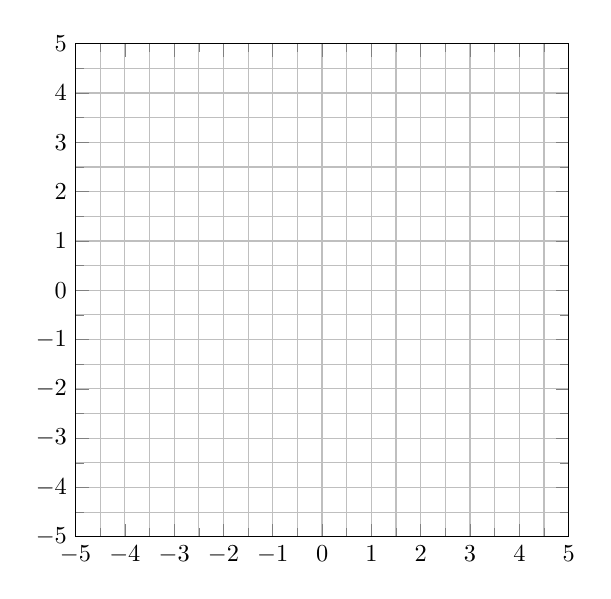
\begin{tikzpicture}[scale=1.1, every node/.style={scale=0.8}]
				\begin{axis}[
						grid=both,
						unit vector ratio=1 1 1,
						ymin=-5,
						ymax=5,
						xmax=5,
						xmin=-5,
						xtick={-10,-9,...,9,10},
						ytick={-10,-9,...,9,10},
						minor tick num=1,
					]
					% \addplot[thick, samples=100,domain=-3:3, name path=A, stealth-stealth]   {-1/2*x+1};
					%  \node[draw,shape=circle, minimum size=2mm,inner sep=0pt,outer sep=0pt, fill=black] at (0,1) {};
					%  \node[draw,shape=circle, minimum size=2mm,inner sep=0pt,outer sep=0pt, fill=black] at (2,0) {};
				\end{axis}
			\end{tikzpicture}
		\end{center}

		\columnbreak

		\begin{enumerate*}[label={(\arabic*)~}, start=2]
			\item $f(x)=\frac{1}{2}x - 1$\hfill\null
		\end{enumerate*}
		\begin{center}
			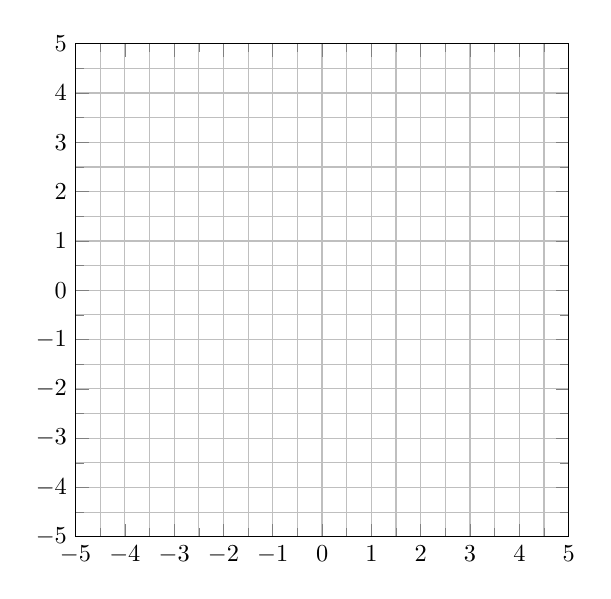
\begin{tikzpicture}[scale=1.1, every node/.style={scale=0.8}]
				\begin{axis}[
						grid=both,
						unit vector ratio=1 1 1,
						ymin=-5,
						ymax=5,
						xmax=5,
						xmin=-5,
						xtick={-10,-9,...,9,10},
						ytick={-10,-9,...,9,10},
						minor tick num=1,
					]
					% \addplot[thick, samples=100,domain=-3:3, name path=A, stealth-stealth]   {-1/2*x+1};
					%  \node[draw,shape=circle, minimum size=2mm,inner sep=0pt,outer sep=0pt, fill=black] at (0,1) {};
					%  \node[draw,shape=circle, minimum size=2mm,inner sep=0pt,outer sep=0pt, fill=black] at (-2,2) {};
					%  \addplot[blue, draw, -stealth] (0, 1)--(0,2) node[midway, xshift=1.5em] {rise=1};
					%  \addplot[red, draw, -stealth] (0, 2)--(-2,2) node[midway, yshift=0.5em] {run=-2};
				\end{axis}
			\end{tikzpicture}
		\end{center}
	\end{multicols}
\end{exercise}
\vspace*{\stretch{1}}
\begin{exercise}
A storage rental company charges a base fee of \$15 and \$$x$ per day for a small cube. Suppose the cost is \$20 dollars for 10 days.
\begin{enumerate}[label={\textup{(\arabic*)~}}]
\item Write the cost $y$ (in dollars) as a linear function of the number of days $x$. 
\item How much would it cost to rent a small cube for a whole summer (June, July and August)?
\end{enumerate}
\end{exercise}

\vspace*{\stretch{3}}
\hfill
\begin{center}
	\raisebox{0.5em}{\rotatebox{\rotationdegree}{
			\parbox{\textwidth}{
				\begin{enumerate*}[label={\theexer~(\arabic*)~}]
					\item $y=0.5x+15$. 
					\item \$61.\hfill\null
				\end{enumerate*}
			}
		}
	}
\end{center}
